%----------------------------------------------------------------------------
\chapter{\caseStudy}
%----------------------------------------------------------------------------

\section{A tanulmány háttere}
Az esettanulmány során egy kitalált, de mégis valósághű vasúti fékrendszert tervezek és elemzem biztonsági szempontból.

A vasútipart és ezzel együtt a vasútifék-technológiát az utóbbi időben rohamos fejlődés határozta meg. 
Számos működési elv elérhető az iparágban (pneumatikus, hidraulikus, elektro-pneumatikus, elektro-hidraulikus, elektromágneses), amelyeknek mind meg van a maga előnye és hátránya.

Ebben a dolgozatban egy összetett integrált fékrendszer megoldást szeretnék modellezni, mely rendelkezik egy fékvezérlő berendezéssel.
Ezért az elavultnak számító és mára leginkább csak a vasúti teherszállításban - az egyszerűsége és költséghatékonysága miatt - használt pneumatikus és a szintén tisztán fizikai elven működő hidraulikus rendszereket nem találtam alkalmasnak a dolgozat témájához.

Napjainkban fontos téma, többek között a globális felmelegedés és a ${CO}_2$ kibocsátás visszaszorítása - melyek részletei és elemzése nem képezik ennek a dolgozatnak részét - miatt, a tömegközlekedés.
A vasútipar emberek szállítmányozására alkamas része is több alrészre bontható, nagysebességű(>300 km/h)/intercity vonatok, 
regionális/ingázó vonatok (pl: Budapesti HÉV), metró, könnyű vasúti vonatok/villamosok.

A dolgozat során egy modern alacsonypadlós városi tömegközlekedésre alkalmas villamos rendszerén keresztül szeretném bemutatni a modell alapú rendszertervezés (Model-based Systems Design, MBSD) módszertanait és az elkészült rendszer biztonsági és megbízhatósági analízisét. 
Mivel az alacsonypadlós villamosokon véges hely áll rendelkezésre, ezért egy kompakt megoldásra van szükség. 
Továbbá, biztosítani kell bármely közlekedési helyzetben a szerelvény biztonságos és optimális lassulását, megállását.

\section{Vasúti jármű fékrendszer} \label{sec:vjfr}
A vasúti járművek fékei rendkívül összetett folyamatot alkotnak és specifikusak a vasúti járművekre.
A fékrendszer egy fontos biztonsági funkció, mely szabályozza a jármű sebességét és megállítja egy fix helyen, mint például egy állomásnál (EN 13452-1, 2003).

Egy vasúti fékrendszernek a következő célokat kell teljesíteni:
\begin{itemize}
    \item Lassítani vagy megállítani a mozgó vonatot
    \item Biztosítani az álló járművet
    \item Kontrollálni a jármű sebességét lejtőn
\end{itemize}

Ezekhez számos funkciót kell teljesítsen a rendszer, melyek a kövezkezők:
\begin{itemize}
    \item üzemi fék
    \item vészfék
    \item biztonsági fék
    \item biztosító fék
    \item parkoló fék
    \item opcionálisan kerékcsúszás prevenciós rendszer (WSP\footnotemark{})
\end{itemize}

\subsection{Üzemi fék}
Az üzemi fék az elsődleges fékrendszer normál üzemi állapotban.
Ezt a rendszert általában a jármű vezetője és/vagy a járművet vezető autómatika kezeli, hogy az általuk kívánt sebességre szabályozzák a vasúti szerelvényt.

\subsection{Vészfék}
Ezen funkció legfőbb célja az utasok, személyzet és a vasutat nem használók biztonságának maximalizálása.
Továbbá ez a funkció képes a lehető leghamarabb nyugalmi állapotba hozni a szerelvényt.

\subsection{Biztonsági fék}
Európában és a világ számos pontján kötelező olyan berendezéssel ellátni az új járműveket, amely a szerelvény esetleges menetközben több részre szakadásakor
a jármű összes részét biztonságosan megállásra kényszeríti. Ezt a funkciót nevezik biztonsági fékmechanizmusnak.

\subsection{Biztosító fék}
Ez a funkció felel a jármű egyhelyben tartásáért, amikor megáll a jármű egy állomáson.

\subsection{Parkoló fék}
A parkoló fék felel a jármű helyben tartásáért, miközben a jármű üzemen kívül van. 

\subsection{Kerékcsúszás prevenciós rendszer}
A WPS\footnotemark[\value{footnote}] egy olyan rendszer, amely optimalizálja a fékteljesítményt és védelmet nyújt a kerék és a sín sérülése ellen gyenge súrlódási viszonyok között.
\footnotetext{Wheelslide Protection System}

\section{Funkcionális dekompozíció}
A \ref{fig:func_arch}. ábrán látható a funkcionális dekompozíciójának block definition diagram-ja.
Ezen látható, hogy a fékrendszer több elemet is támogat a \ref{sec:vjfr}. részben taglalt funkciók közül.
A rendszer a következő öt funkciókkal rendelkezik, ahogy az a \ref{fig:func_arch}. ábrán is látható: 
(1) üzemi fék (service brake), 
(2) vészfék (emergency brake), 
(3) biztonsági fék (security brake),
(4) parkoló fék (parking brake) és 
(5) kerékcsúszás gátlás (wheelslide protection).
Továbbá az ábrán az is látható, hogy a fékrendszer képes forgóvázra nehezedő súly által szabályozni a fékezési erőt.

\begin{figure}
    \footnotesize
    \centering
    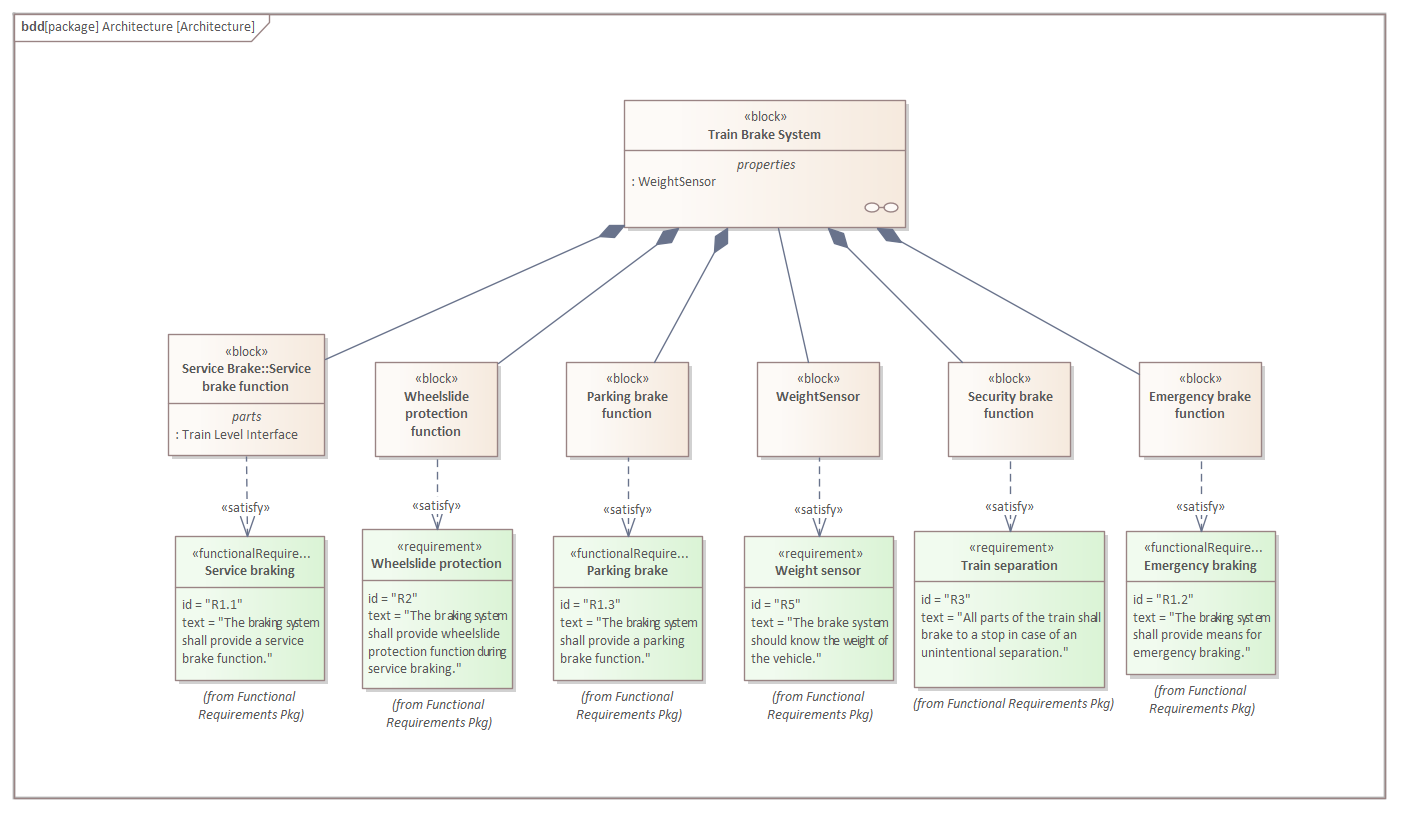
\includegraphics[width=150mm, keepaspectratio]{figures/Architecture.png}
    \caption{A tervezett fékrendszer funkcionális dekompozíciója}
    \label{fig:func_arch}
\end{figure}

Az \ref{fig:func_arch_ibd}. ábrán látható a rendszer belső felépítése (IBD\footnote{internal block diagram}).
Az ábra tartalmazza és definiálja az alrendszerek kapcsolatát, továbbá leírja a rendszer külső csatlakozási pontjait portok által.
\begin{figure}
    \footnotesize
    \centering
    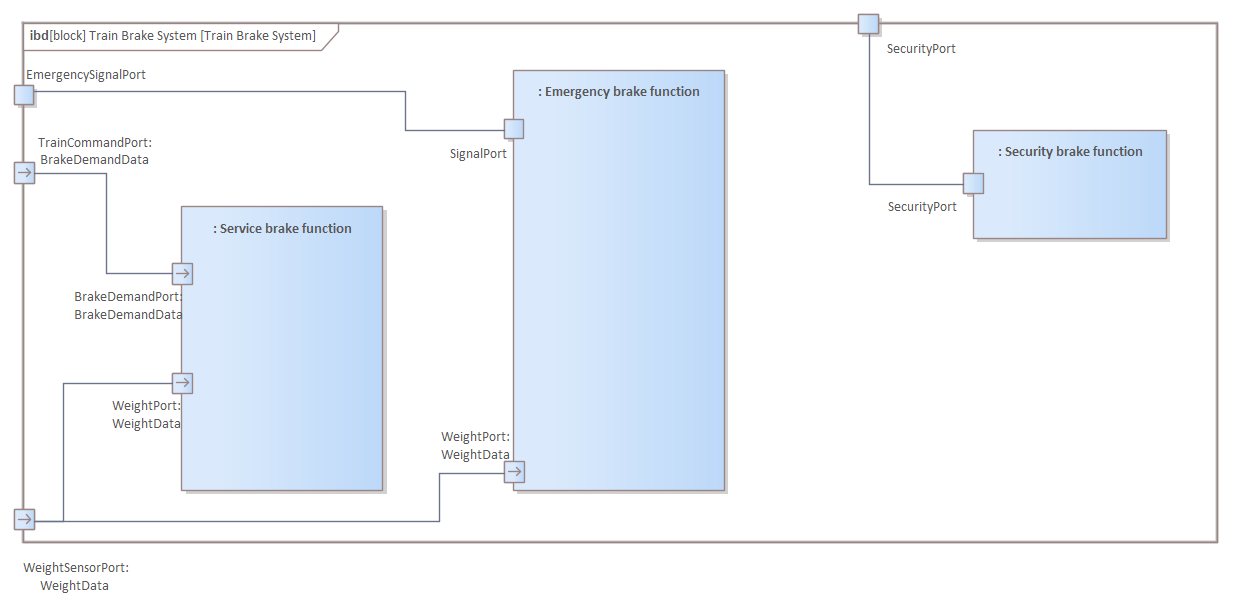
\includegraphics[width=150mm, keepaspectratio]{figures/Architecture_ibd.png}
    \caption{A fékrendszer belső felépítése}
    \label{fig:func_arch_ibd}
\end{figure}

\subsection{Üzemi fék}
Az dekompozíciós folyamatot az üzemi fék alrendszeren folytatva az \ref{fig:service_brake_bdd}. ábra mutatja az üzemi fék funkcionális felbontását/BDD\footnote{Block Definition Diagram}-jét.
Az ábrán látható, hogy ez egy vezérlő funkció ezért megjelenik a vezérlő-rendszer-visszacsatoló hármas a modellben.
Továbbá az is látszik, hogy a vezérlő funkció egy összetett eleme az alegységnek.

\begin{figure}
    \footnotesize
    \centering
    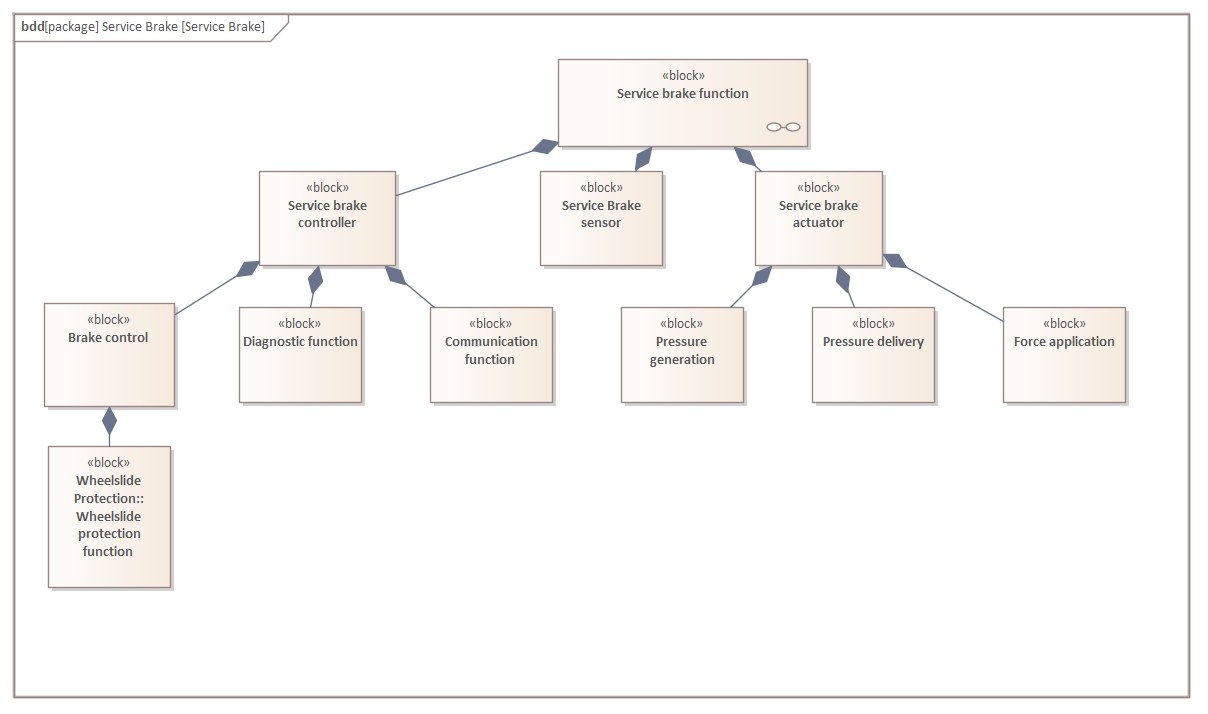
\includegraphics[width=150mm, keepaspectratio]{figures/Service_Brake_bdd.png}
    \caption{Üzemi fék blokk definition diagramm-ja.}
    \label{fig:service_brake_bdd}
\end{figure}

